<<<<<<< HEAD
\section{Background}

\subsection{Disaggregated Memory}

Memory disaggregation separates primary storage from the CPU
by a fast network. The question \textit{how to present
memory over the network to an application?} is still open,
and a spectrum of system designs currently exist.
Transparent systems present far memory to the application as
if it were local. Virtual memory enables paging systems to
keep a cache of local pages, and swap in and out
transparently on page faults ~\cite{infiniswap, leap,
fastswap}.  Some have argued that page granularity is too
course and built upon an incoherent caching
layer~\cite{kona,legoos}.  In both cases transparency
incurs a performance cost as remote accesses cannot be
optimized for by the running application.
%%
Alternatively applications can access remote memory
explicitly with an API similar to an RPC
call~\cite{aifm,reigons,clover,sherman,faast}. Explicit
access allows for optimized remote requests. They can be
batched, scheduled, and managed by libraries and runtimes. 
%%
Whether explicit or transparent sharing is expensive, at the
time of writing no transparent system supports shared memory
-- the cost of cache coherence is prohibitively high in
terms of bandwidth and latency. Explicit cases are more
promising for sharing as they allow application developers
to acquire locks, and for libraries to make use of
optimistically concurrent datastrcutrues.

\subsection{RDMA protocol}

RDMA provides an interface for accessing remote memory. It
provides a set of zero copy instructions (\textit{verbs})
which are initiated by a client cpu. NICs manage the entire
network stack including control flow, reliable delivery, and
at most once semantics. The guarantees RDMA provides are
configurable -- connection's UDP like semantics are provided
by Unreliable Datagram (UD) and Unreliable Connections (UC),
while Reliable Connections (RC) at similar to TCP, ensuring
in order delivery, and enabling RDMA's one-sided operations
Read, Write, and Compare and Swap (CAS).

Which connections to use is an intense topic for debate.
Reliable connections use NIC memory, a precious resource,
and projects designed using Mellanox CX3-CX5 noted that RC
bottlenecked scalability due to memory and cache
limitations~\cite{farm,faast,erpc,lite,design-guidelines}.
While host memory can provide better scalability modern NICs
have bigger caches with better cache
management~\cite{storm}. In the disaggregated setting no
memory side CPU exists to manage the state making RC the
only option for one sided operations.

\todo{connection multiplexing ~\cite{flock}}
\todo{RDMA middlebox (find citaitons ~\cite{mind,switchml})}

%% RDMA

% Remote direct memory access (RDMA) is a network protocol
% which allows NICs to bypass CPUs and access host memory
% directly.  The RDMA protocol consists of a set of verbs
% which abstract remote memory instructions. Instruction
% execution and connection state are entirely managed by the
% NIC which exposes the verbs API to the CPU. The CPU
% registers memory regions for DMA with the NIC and sets up
% connections (Queue Pairs) with a remote RDMA enabled NIC.
% %%
% RDMA connections come in a variety of flavors, each of which
% enables a different set of RDMA verbs and delivary
% guarantee~\cite{herd, erpc, storm}. Unreliable Datagram
% (UD), and Unreliable Connection (UC) operate similar to UDP
% with no reliable delivery or ordering guarantees and a
% restricted set of verbs.  Reliable Connected (RC) operates
% similar to TCP, the NIC manages connection states for each
% QP and ensures reliable in-order delivery by using sequence
% numbers and a go-back-n retransmission protocol.
% %%
% Serious debate exists over which connections to
% use~\cite{storm,cell,herd,faast,farm}, each has advantages
% and disadvantages in terms of NIC resource utilization,
% throughput, and latency. Disaggregated architectures have no
% remote CPU's, in this proposed setting RC is the most
% attractive as it alone enables the use of one-sided verbs
% :\textit{Read}, \textit{Write}, and the atomic \textit{CAS}
.


%% RDMA Connections
%% RDMA Atomics

\subsection{Programmable Switches} Most proposals for
disaggregation are at rack-scale. They propose a single rack
with servers partitioned into roles: compute, memory, and
storage, each of which is interconnected by a TOR.  The TOR
is central in this architecture, a fact which has not gone
unnoticed by system designers who argue that a programmable
switch can facilitate remote memory APIs, and OS
functionality~\cite{disandapp,mind}. 
%%
Literature on offloading OS, and service level functionality
to programmable switches is
plentiful~\cite{netlock,netkv,netchain,netcache}. The
constraints in each case are similar, switches have limited
memory, and processing capabilities, if the computational
ask of the switch is too high packets must be recirculated
adding additional latency, and reducing aggregate bandwidth.
Ideal applications for programmable switches use little
memory, require little processing and enable a huge
performance benefit from centralization, and the billions of
operations (in terms of packets) that a switch can process
per second.
%%
Prior work has shown that programmable switches are able to
manage locks~\cite{netlock}, track the state required to
maintain an RDMA reliable connection~\cite{tea}, and provide
rack scale serialization at low
cost~\cite{eris,no,when-computer}. These properties make a
top-of-rack programable switch ideal for managing remote
memory as it can guard access, maintain connections, and
provide serialization primitives for all clients.


=======
>>>>>>> 57acc706317134a206acb9152f2c868c3f9ec0d9
% \section{Serialization}

% \begin{figure}[t]
%   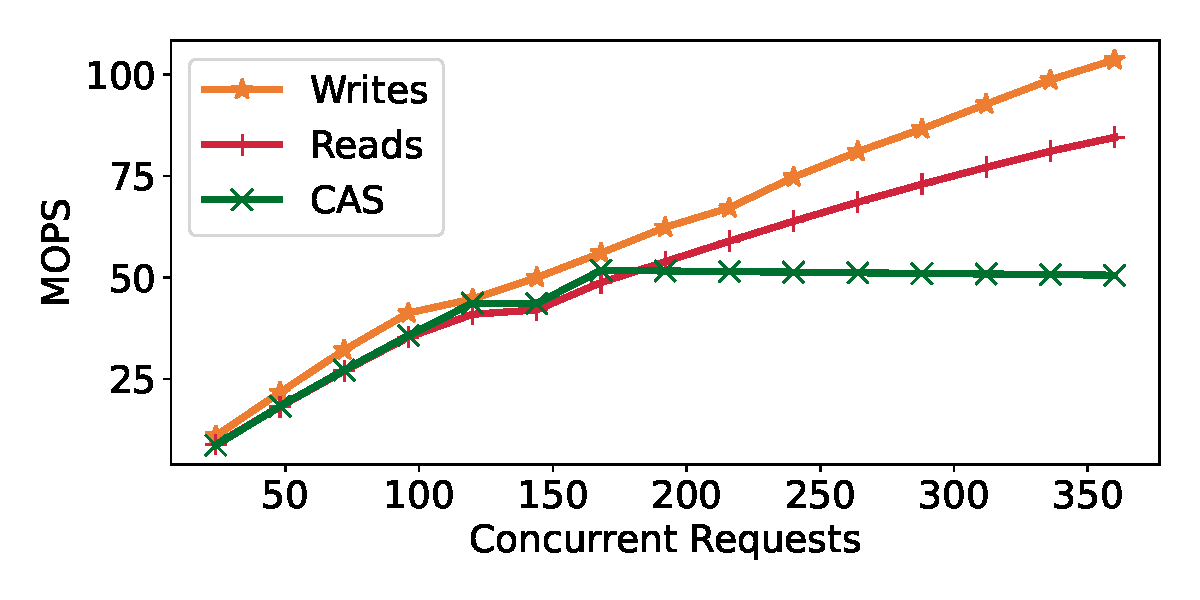
\includegraphics[width=0.485\textwidth]{fig/rdma_concur.pdf}
%   \vskip -0.5em

%     \caption{Achieved throughput of RDMA verbs across twenty queue
%       pairs on data-independent addresses as a function of request
%       concurrency.  When using atomic requests, ConnectX-5 NICs can
%       support approximately 2.7 MOPS per queue pair, up to about 55
%       MOPS in aggregate.}

%     \label{fig:rdma_concur}
%       \vskip -0.5em
% \end{figure}

% \begin{figure}[t]
%     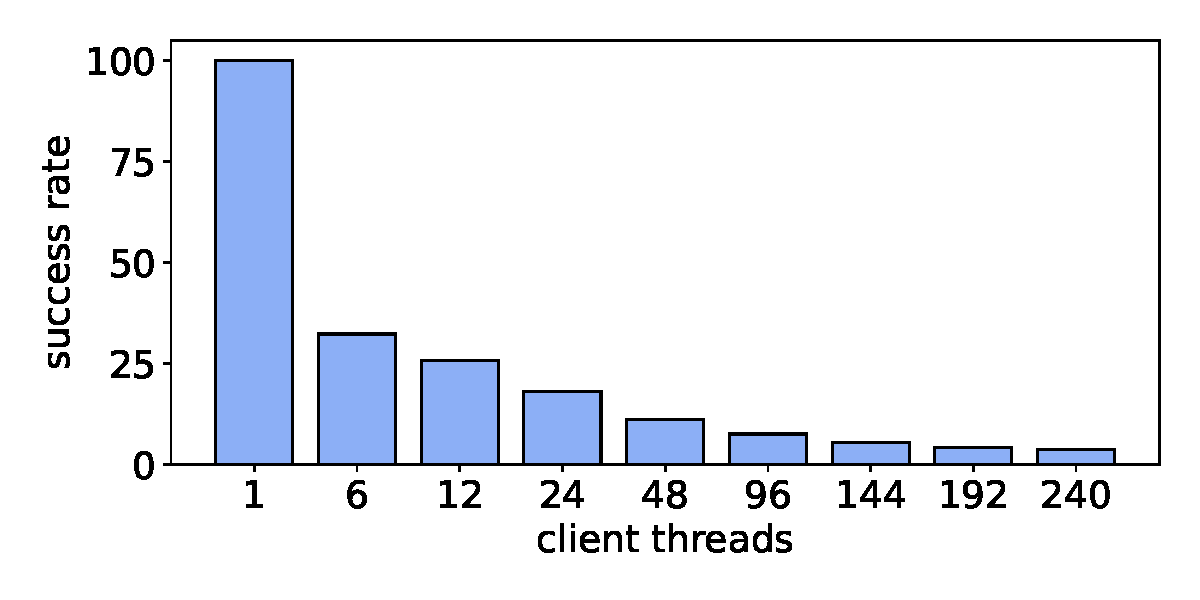
\includegraphics[width=0.485\textwidth]{fig/success_rate.pdf}
%     \vskip -0.5em
%     \caption{Percentage of successful operations in a
%       50:50 read-write workload spread across 1,024 keys according
%       to a Zipf(0.99) distribution as more client threads are
%       added. At 240 threads less than 4\% of operations succeed.}
      
%     \vskip -0.5em
%     \label{fig:success_rate}
% \end{figure}

% \begin{figure}[t]
%   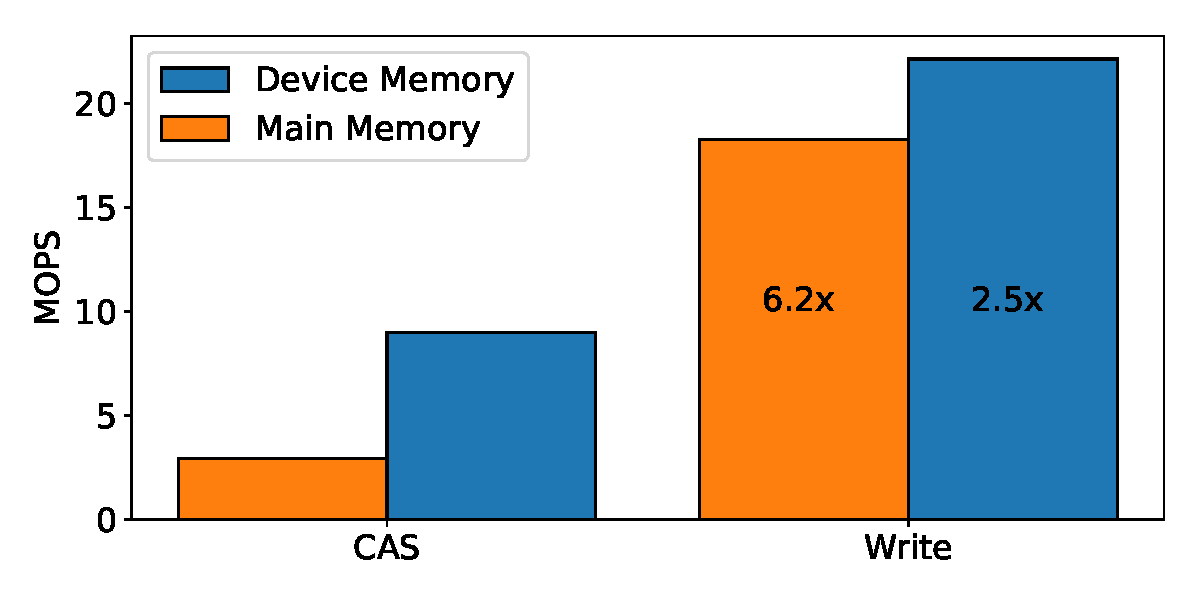
\includegraphics[width=0.485\textwidth]{fig/cas_vs_writes.pdf}
% %  \vskip -0.5em

%   \caption{ Throughput comparison of serialized RDMA operations in
%     NIC-mapped device and main memory. Writes obtain 6.2$\times$ higher
%     throughput than CAS in host memory and 2.5$\times$ higher in NIC memory despite being restricted to a single queue pair.  }

%     \label{fig:cas_vs_writes}
% %      \vskip -0.5em
% \end{figure}

% \subsection{RDMA serialization} 
% %%
% RDMA atomics instructions serialize remote memory operations
% without the need for a memory side CPU. These instructions
% \textit{Fetch-and-Add} and \textit{Compare-and-Swap} (CAS)
% execute on 64 bit width words and are guaranteed to have
% atomic visibility across all queue pairs. These operations
% are expensive. On a single address atomic instructions can
% only execute a few million operations per second, each
% operation forces a blocking PCIe round trip.  As a
% performance mitigation Mellanox NICs supply a small (few KB)
% region of device mapped memory which allows the memory side
% NIC to execute RDMA instructions on it's local device memory
% without incurring a PCIe round trip~\cite{sherman}.
% Executing atomics on this memory is 3x higher throughput
% than host memory, but still slower than it's read and write
% counterparts~\ref{fig:cas_vs_writes}.  Across independent
% addresses they have approximately half the throughput of
% read and write (Figure~\ref{fig:rdma_concur}).

% Data structures built on RDMA atomics have hard performance
% limits because the aforementioned constraints.  Locks
% located at a single address which use traditional lock,
% unlock operations are limited to around 500k accesses per
% second. This assumes perfectly coordinated requests, under
% contention requests which fail to acquire or release a lock
% still consume operation bandwidth.
% %%
% Under contention RDMA has poor support for traditional
% locking. In contrast optimistic data structures with locks
% scattered throughout, such as a linked list, are not rate
% limited by this single address restriction.  However, they
% are fundamentally limited by the fact that any atomics have
% half the throughput of reads and writes. More critically,
% under contention optimistic data structures have no liveness
% guarantees. We measure the failure rate of optimistic reads
% and writes to a shared linked list. Operations are reads and
% writes to the tail of the list, all writes are appends.
% under contention atomic operations fail frequently
% (Figure~\ref{fig:success_rate}).  RDMA has no support for
% resolving pointers (pointer chasing) and retrying operations
% for such data structures~\cite{rma,snap,prism}, a simple
% operation usually executed by a memory side CPU. As such
% RDMA clients are forced to resolve their failures requests
% themselves often retrying many times.
% %%
% Atomic operations are not the only serialization mechanism
% provided by RDMA. Reliable Connections provide in order
% delivery on individual queue pairs. This allows clients to
% issue multiple requests in parallel and allows the NIC to
% resolve reordering and dropped packets using go-back-n
% retransmission.  When clients are collocated, queue pairs
% can be shared by multiple cores through techniques such as
% flat combining~\cite{flock,sherman}. Flat combing removes
% the need for RDMA atomics, as clients can locally resolve
% their conflicts and then issue their requests as reads and
% writes.  Unfortunately this technique is not applicable to
% distributed clients as they do not share access to the same
% queue pair.


% \subsection{Overheads}

% \paragraph{Bandwidth inflation.} 
% %%
% One of the most direct impacts of failed requests is the
% bandwidth overhead of the retries. When atomic operations
% fail they must be retried.  In the case of locking the
% number of retries is a direct result of the critical section
% size, the number of clients, and the aforementioned
% operation limits. Each failed request consumes additional
% bandwidth. Bandwidth inflation in optimisitic schemes is
% proportial to the degree of contention. When optimistic
% operations fail they must be retried.
% %%
% Our measurements show that under contention the average
% bandwidth cost of Clover read and write operations can
% inflate by 16$\times$ (Figure~\ref{fig:bandwidth_reduction})
% when compared to an optimal scenario in which all operations
% succeed on their first try.

% % Because a Clover operation actually
% % consists of multiple RDMA requests, the total bandwidth is not
% % strictly proportional to the failure rate, but rather slightly
% % sub-linear.  Nevertheless, the expected cost of each operation rises
% % steadily with contention, which is a function of both the workload and
% % level of concurrency. 

% \paragraph{Tail latency.}

% Perhaps even more significant than the overheads associated with the expected
% number of retries is the cost at the tail---namely the latency associated with
% those particularly ``unlucky'' requests that fail repeatedly.  Note that these
% operations are precisely those for hot memory locations, so likely to be
% ones that matter.  Under contention
% %(e.g., 50\% write operations with 396 threads)
% Clover's 99th-percentile tail latency increases by
% over 300$\times$ (Figure~\ref{fig:tail_latency}) in our experiments.

% % \subsection{Programmable Switch Serialization}
% \section{In-network serialization}

% \begin{figure}[t]
%     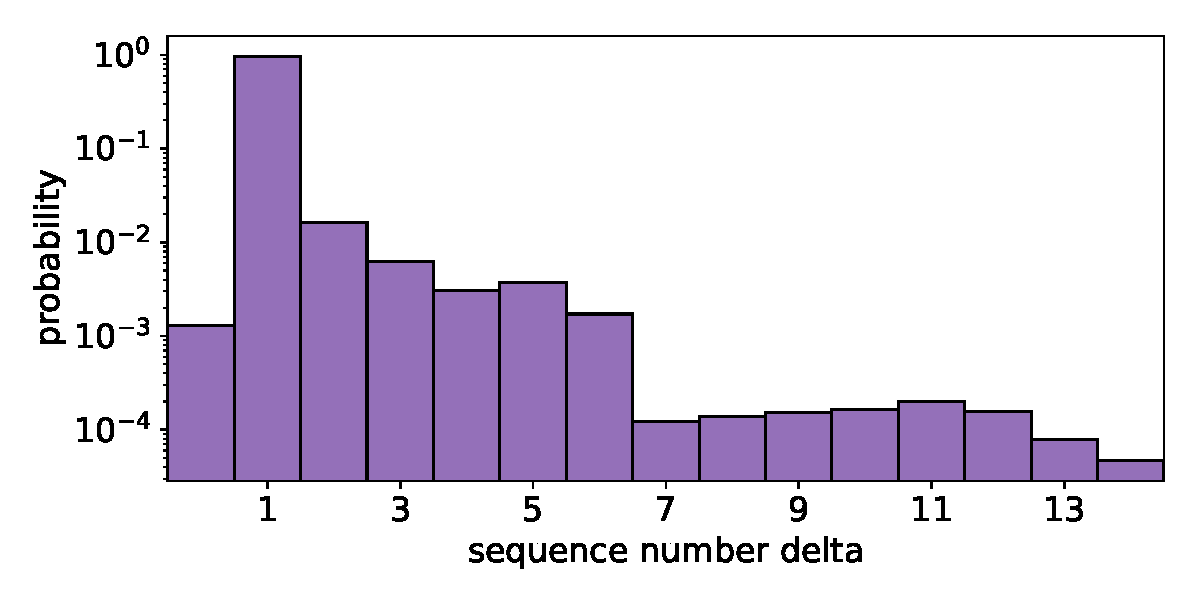
\includegraphics[width=0.485\textwidth]{fig/qp_reordering.pdf}
%   \vskip -0.5em    
%     \caption{PDF of request reorderings.  Retransmitted requests lead to reordering values of zero.   97\%
%     of requests retain their order (delta=1), however reorderings of up to 15
%     requests can occur. (Note logarithmic $y$ axis.)}
%   \vskip -0.5em
%     \label{fig:reorder}
% \end{figure}

% Switches can cheaply serialize packets~\cite{when-computer}.
% Programable switches with P4 pipelines can utilize this
% cheap serialization, along with their ability to manage
% small amounts of state in network, to serialize distributed
% applications. Mind for instance provides a unified TLB and
% cache for disaggregated applications~\cite{mind}. Packets
% processed by a programmable switch are sequenced in order,
% updates to the switches registers are atomic with respect to
% the packets as each state of the pipeline is occupied by
% exactly one packet at a time. A centralized switch can
% therefore apply monotonic sequence numbers to a stream of
% packets, maintain a lock, or keep a shared variable up to
% date without the need for explicit atomic operations.

% Unfortunately this serialization is not sufficient for RDMA
% memory operations out of the box. RDMA packets on two
% reliable connections may be ordered on the switch, and then
% subsequently reordered by the receiving side NIC, or by the
% PCIe bus~\cite{understanding-pcie}. NIC and PCIe reordering
% is not merely an academic concern!  Figure~\ref{fig:reorder}
% illustrates the extend of reordering across connections.
% This experiment uses an in network serializer to give each
% packet an incremental monotonic sequence number. The x axis
% measure the absolute delta between sequence number values on
% response packets.  The majority of packets remain ordered
% (sequence number 1), however significant reordering does
% occur up to 15 packets apart.

% Switches are not intended to be general purpose computers,
% their purpose is to forward packets. It is trivial to
% construct switch programs which consume it's few resources.
% Oversized caches step on the toes of packet buffers and lead
% to dropped packets, and complex logic requires packet
% recirculation which eats into the switches bandwidth.
% limiting it's ability to buffer, and process packets at full
% bandwidth.
% %%
% For example, terminating connections with a switch is
% prohibitively expensive as both the state of the entire
% connections, and the logic for connection startup and
% teardown would consume large quantities of the switches
% buffers. Any logic, or data offloaded to a programable
% switch must therefore be minimal in order to meet the
% compute and data restrictions of the switches SRAM.


\section{Serialization}

The fundamental challenge faced by passive remote memory systems is
ensuring consistency~\cite{ivy} by ordering accesses to any given
location.  RDMA reliable connections provide per-connection ordering,
enabling clients to
%Atomic operations are not the only serialization mechanism
%provided by RDMA. Reliable Connections provide in order
%delivery on individual queue pairs. This allows clients to
issue multiple outstanding requests; the NIC ensures in-order delivery despite 
packet reordering and drops with sequence numbers and go-back-$n$
retransmission.  When clients are collocated, queue pairs
can be shared by multiple cores through techniques such as
flat combining~\cite{flock,sherman}.
%Flat combing removes
%the need for RDMA atomics, as clients can locally resolve
%their conflicts and then issue their requests as reads and
%writes.
Unfortunately this technique is not applicable to
distributed clients that cannot share connections.
In this section we experimentally illustrate the challenges to
ordering across such clients.


% \subsection{Programmable Switch Serialization}
\subsection{Switch-enforced ordering}

\begin{figure}[t]
    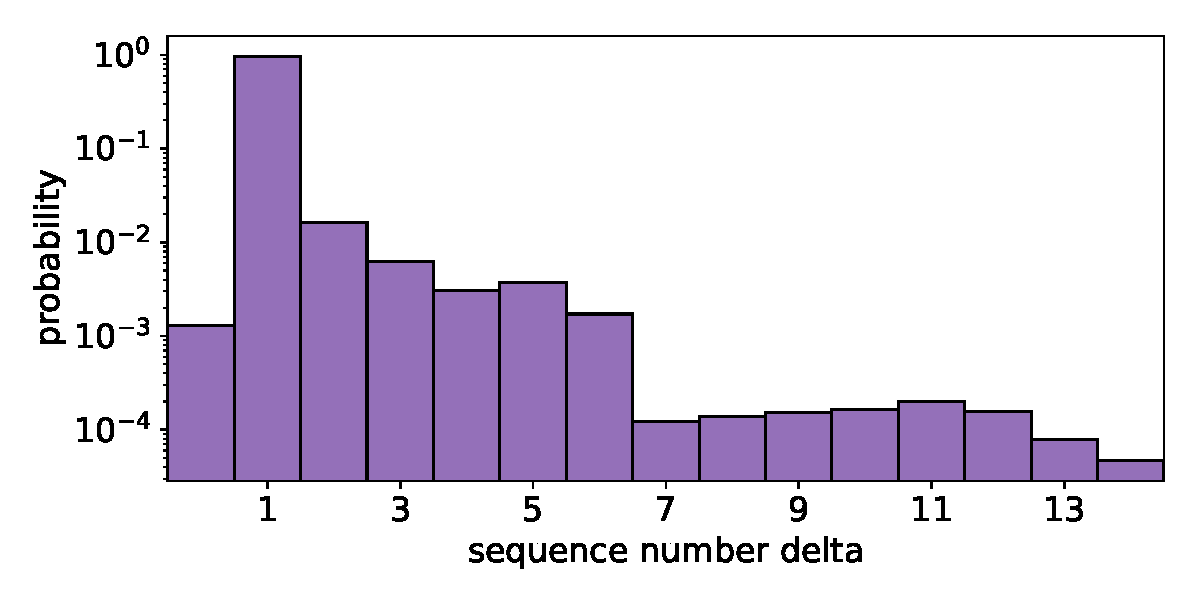
\includegraphics[width=0.485\textwidth]{fig/qp_reordering.pdf}
  \vskip -0.5em    
    \caption{PDF of request reorderings.  Retransmitted requests lead to reordering values of zero.   97\%
    of requests retain their order (delta=1), however reorderings of up to 15
    requests can occur. (Note logarithmic $y$ axis.)}
  \vskip -0.5em
    \label{fig:reorder}
\end{figure}

Packets processed by a programmable switch pipeline are sequenced in
order: updates to switch registers are atomic as each state of a
pipeline is occupied by exactly one packet at a time.  Moreover, all
packets destined to a given port must traverse the same egress
pipeline.  As a result, the ToR places packets from all flows destined
to the same (single-homed) destination in a total order---not only with
respect to their own flow, but others as well.  
%% switch can therefore apply monotonic sequence numbers to a stream of
%% packets, maintain a lock, or keep a shared variable up to date without
%% the need for explicit atomic operations.
%
In the context of RDMA, however, switch-enforced packet ordering is
insufficient.  Even if packets (from various reliable connections)
arrive at a server NIC in a given order, they may (appear to) be
processed in arbitrary order due to contention at the NIC or PCIe
bus~\cite{understanding-pcie}.

Figure~\ref{fig:reorder} shows that NIC
and PCIe reordering is not merely an academic concern, but occurs with
some frequency.  In this example, we issue RDMA read, write and CAS
requests at a rate of one million requests per second to 1,024
different memory locations according to a Zipf distribution and spread
these requests across 32 different reliable connections. Each request is routed
through a programamble switch that keeps a global request counter for
each RDMA request (i.e., ground truth regarding request ordering). We
track the order of responses relative to the order the corresponding
request was issued from the middlebox. The plot shows the distribution
of sequence-number gaps between responses. As expected, the vast
majority differ by one (i.e., the same order they were dispatched from
the switch), but a non-trivial number are out of order by one to five
requests, and some by up to 15.  Moreover, this experiment neglects
the reality that some fames may be corrupted and/or lost by the link,
necessitating retransmission and further cross-flow reordering.

%% Figure~\ref{fig:reorder} illustrates the extent
%% of reordering across connections.  This experiment uses an in network
%% serializer to give each packet an incremental monotonic sequence
%% number. The x axis measure the absolute delta between sequence number
%% values on response packets.  The majority of packets remain ordered
%% (sequence number 1), however significant reordering does occur up to
%% 15 packets apart.





\subsection{Atomic RDMA operations} 

While the RDMA protocol does not have a mechanism to enforce
cross-flow ordering, it provides atomic verbs that allow applications
to implement their own mechanisms to detect races and/or enforce
ordering.  The 1-sided \textit{Fetch-and-Add} and
\textit{Compare-and-Swap} (CAS) operations target 64-bit words in
remote memory.  Like their traditional CPU counterparts, atomic
requests appear to execute at a single point in time, ensuring a total
ordering on all data-dependent instructions and a partial ordering
between all other instructions---i.e., all other instructions appear
to occur strictly before or after the atomic, regardless of whether
they are themselves atomic.  Remote memory systems can use these
atomic operations in two basic ways to enforce consistency: implement
shared locks or optimistic concurrency control.

\begin{figure}[t]
  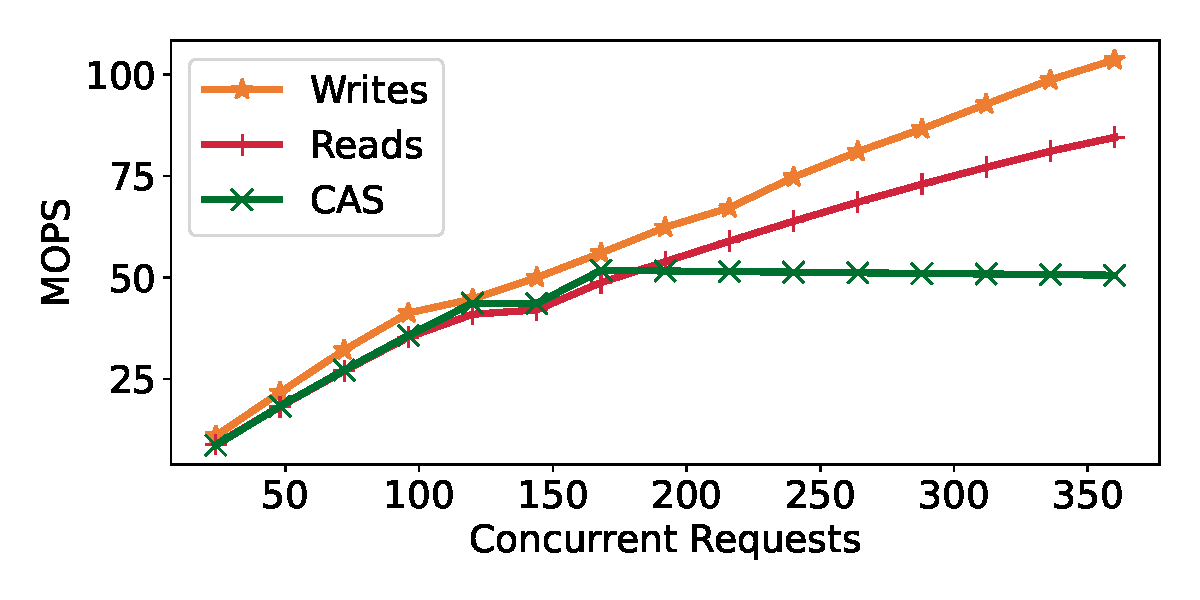
\includegraphics[width=0.485\textwidth]{fig/rdma_concur.pdf}
  \vskip -0.5em

    \caption{Achieved throughput of RDMA verbs across twenty queue
      pairs on data-independent addresses as a function of request
      concurrency.  When using atomic requests, ConnectX-5 NICs can
      support approximately 2.7 MOPS per queue pair, up to about 55
      MOPS in aggregate.}

    \label{fig:rdma_concur}
      \vskip -0.5em
\end{figure}

\begin{figure}[t]
  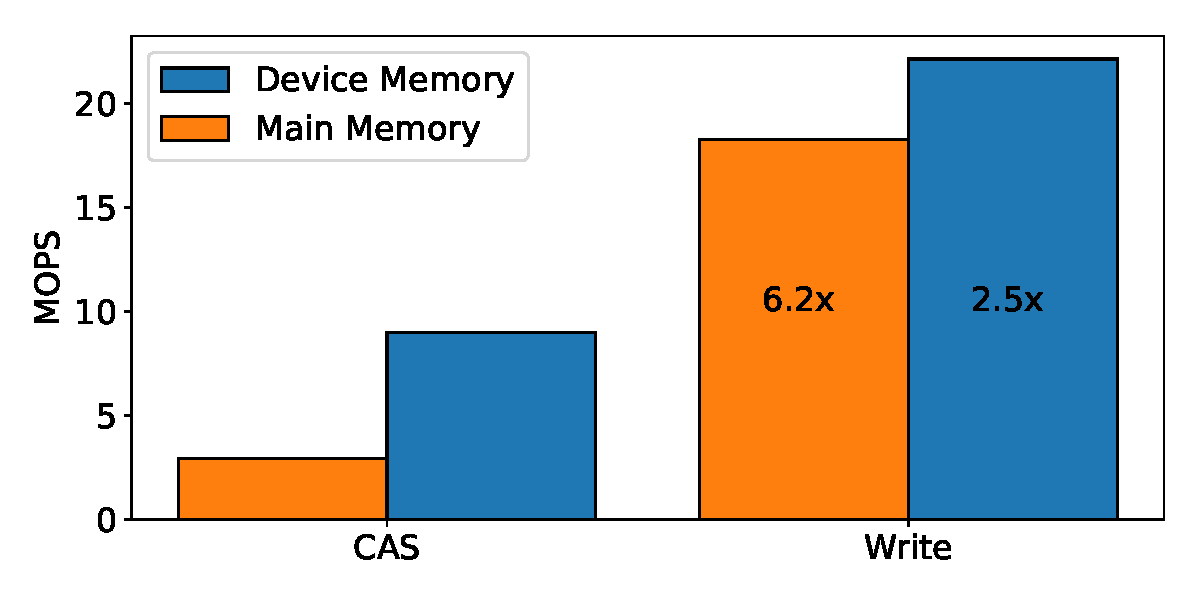
\includegraphics[width=0.485\textwidth]{fig/cas_vs_writes.pdf}
%  \vskip -0.5em

  \caption{ Throughput comparison of serialized RDMA operations in
    NIC-mapped device and main memory. Writes obtain 6.2$\times$ higher
    throughput than CAS in host memory and 2.5$\times$ higher in NIC memory despite being restricted to a single queue pair.  }

    \label{fig:cas_vs_writes}
%      \vskip -0.5em
\end{figure}

\paragraph{Remote locks}
In a remote-locking scheme, clients use an atomic RDMA operation to
attempt to aquire a lock: because the operations are totally ordered
at most one client will succeed at a time.  Unfortunately, atomics are
famously expensive~\cite{design-guidelines}, fundamentally because
they require mutual exclusion across all RDMA queue pairs---concurrent
read and write operations with a data dependency on the atomic address
must stall until the atomic completes.  Figure~\ref{fig:rdma_concur}
considers the best-case scenario where clients attempt to access
unique locks (i.e., each instruction is issued to an
isolated cache line) in remote memory using an atomic operation in
comparison to reads and writes.  We confirm that the findings of prior
studies~\cite[Fig. 14]{design-guidelines} with older hardware (i.e.,
ConnectX-3) remain true on our ConnectX-5 NICs, namely that atomic
requests scale with non-atomics only to a point.\footnote{Experiments
with a ConnectX-6 exhibit similar behavior.}  CAS operations have a
hard performance ceiling, while standard verbs (e.g., read and write)
continue to scale with increased request concurrency.  The situation
is even worse when operations target the same address (i.e., lock
contention; not shown).

%% These operations are expensive. On a single address
%% atomic instructions can only execute a few million operations per
%% second, each operation forces a blocking PCIe round trip.  As a
%% performance mitigation Mellanox NICs supply a small (few KB) region of
%% device mapped memory which allows the memory side NIC to execute RDMA
%% instructions on it's local device memory without incurring a PCIe
%% round trip~\cite{sherman}.  Executing atomics on this memory is
%% 3$\times$ higher throughput than host memory, but still slower than
%% it's read and write counterparts~\ref{fig:cas_vs_writes}.  Across
%% independent addresses they have approximately half the throughput of
%% read and write (Figure~\ref{fig:rdma_concur}).

\begin{figure}[t]
    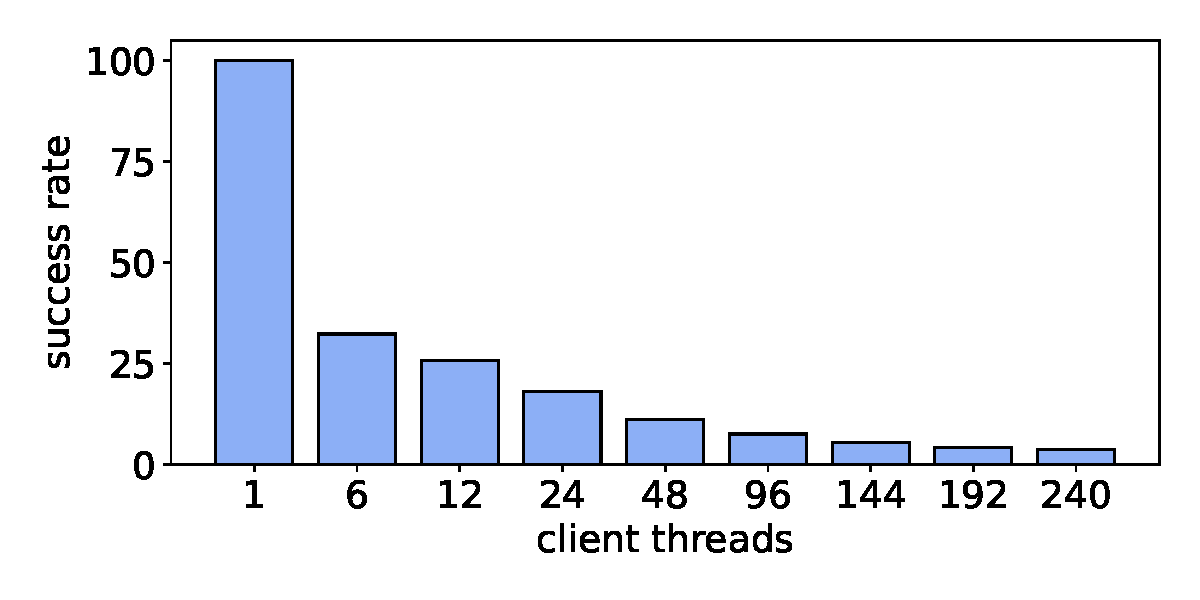
\includegraphics[width=0.485\textwidth]{fig/success_rate.pdf}
    \vskip -0.5em
    \caption{Percentage of successful operations in a
      50:50 read-write workload spread across 1,024 keys according
      to a Zipf(0.99) distribution as more client threads are
      added. At 240 threads less than 4\% of operations succeed.}
      
    \vskip -0.5em
    \label{fig:success_rate}
\end{figure}

One of the difficulties RDMA NICs face when implementing atomic operation
is ensuring that there are no other conflicting memory operations at
the server---even ones issued locally.  More generally, any
main-memory operation issued by the NIC must cross the PCIe bus and
face potential contention.  Modern Mellanox NICs like the ConnectX-5
provide a small region of on-NIC memory that can be mapped into the
address space of RDMA applications,
%.  Mapping RDMA requests onto NIC memory
removing the remote PCIe overhead for frequently accessed data.
(Indeed, Sherman employs this memory region to store its B+Tree locks.)
%but still requires atomicity across queue pairs.
Figure~\ref{fig:cas_vs_writes} compares the performance of
serialized CAS and write operations to addresses in main vs.
NIC-hosted device memory. CAS operations are issued across many
queue pairs to achieve maximum throughput while the write operations are
issued on a single queue pair to enforce serialization.
%leverage the serialization provided
%by RDMA's reliable connection abstraction to ensure in-order
%execution.
While the use of NIC-hosted memory boosts CAS throughput
from approximately 3 to around 9 MOPS, write operations remain
dramatically more efficient in either case.

\paragraph{Optimistic concurrecy.}
One way to avoid the overhead of remote lock aquisition in low-load
situations is to attempt to directly modify the data (using an
atomic RDMA operation) and recover if the operation fails due to a
race; such schemes are known as optimistic concurrency control.  While
far more performant than lock-based appraoches in the un-contended
case, optimistic appraoches can be prohibitively expensive when
contention is common.  As a concrete example we consider the chances
of success in Clover.
%Recall Clover maintains a linked list for each key and attempts to read and
%write to the tail of the list for each operation. The location of the tail of
%the list is cached at each client and used as a hint for subsequent operations.
%If the hint is stale the client obtains an updated tail pointer and retries the
%RDMA request.
Figure~\ref{fig:success_rate} shows the percentage of requests
which succeed in a 50:50 read-write workload as a function of the number of
concurrent client threads. Success rate drops dramatically as client threads
increase.

At present RDMA has no support for addressing failed operations at the
server, such as pointer chasing or retrying operations---although some
have proposed such extensions~\cite{rma,snap,prism}.  Rather, RDMA
clients are forced to resolve failures themselves at significant cost.
%In general, the conflicting operation(s)
%must be retried incurring additional latency and bandwidth.
In some
systems, the retry is a heavyweight, pessimistic operation, leading to
a substantial---but fixed---overhead.  In others, like Clover,
subsequent attempts remain optimistic, resulting in a linear
(per-retry) increase in costs.  In the latter case, very high
rates of contention can lead to congestion collapse, where a retry is
essentially doomed to failure, dramatically decreasing system
throughput.
%

%\paragraph{Bandwidth inflation.} 

Concretely,
%One of the most direct impacts of failed requests is the bandwidth
%overhead of the retries.  Because a Clover operation actually
%consists of multiple RDMA requests, the total bandwidth is not
%strictly proportional to the failure rate, but rather slightly
%sub-linear.  Nevertheless, the expected cost of each operation rises
%steadily with contention, which is a function of both the workload and
%level of concurrency.  Our
our measurements show that under contention the
average bandwidth cost of Clover read and write operations can inflate
by 16$\times$ (Figure~\ref{fig:bandwidth_reduction}) when compared
to an optimal scenario in which all operations succeed on their first
try.
%
%\paragraph{Tail latency.}
%
Perhaps even more significant than the overheads associated with the expected
number of retries is the cost at the tail---namely the latency associated with
those particularly ``unlucky'' requests that fail repeatedly.  Note that these
operations are precisely those for hot memory locations, so likely to be
ones that matter.  Under contention
%(e.g., 50\% write operations with 396 threads)
Clover's 99th-percentile tail latency increases by
over 300$\times$ (Figure~\ref{fig:tail_latency}) in our experiments.



\subsection{Implications}

Systems that leverage RDMA atomics have hard performance
limits because the aforementioned constraints.  Locks
located at a single address which use traditional lock,
unlock operations are limited to around 500k accesses per
second. This assumes perfectly coordinated requests, under
contention requests which fail to acquire or release a lock
still consume operation bandwidth.
%%
Under contention RDMA has poor support for traditional
locking. In contrast optimistic data structures with locks
scattered throughout, such as a linked list, are not rate
limited by this single address restriction.  However, they
are fundamentally limited by the fact that any atomics have
half the throughput of reads and writes. More critically,
under contention optimistic data structures have no liveness
guarantees.

%% We measure the failure rate of optimistic reads
%% and writes to a shared linked list. Operations are reads and
%% writes to the tail of the list, all writes are appends.
%% under contention atomic operations fail frequently
%% (Figure~\ref{fig:success_rate}).

%%



\section{\sword}

We present {\sword} a middlebox solution for sharing remote
memory. {\sword} enables sharing by providing two forms of
application specific serialization. The first of which is to
resolve atomic operations in network. Using a cache \sword
determines the result of the atomic operation, and forwards
the result to memory as a write. The semantics of RDMA RC
connections are used to ensure that the result of the
resolved atomic arrives in far memory in order. Second
{\sword} can remove contention from optimistic data
structures through steering. \sword caches updates to the
shared structures and modifies stale requests in flight with
the most up to date information removing the need for
operations to fail. These mechanisms are used to accelerate
locks in Sherman~\cite{sherman} and remove all contention
from a key-value store, Clover~\cite{clover}.
%%
These
techniques are implemented in a DPDK prototype for the lock
based approach and fully realized in P4 for optimistic data
structures. Figure~\ref{fig:system} shows the overall design
of {\sword}.

% Locks are
% managed in network, and the results of locking operations
% are forward to memory. Lock accesses are accelerated by
% replacing RDMA atomic operations with writes in flight.
% Modified lock operations are multiplexed onto existing RDMA
% connections, per lock, to ensure serialized access to the
% lock. {\sword} also provides a mechanism to remove
% contention from optimistic data structures by caching the
% metadata required to detect and resolve conflicts. 

% In all cases switch memory and compute are highly
% constrained. Any operations that exceed the processing
% limit of the match action pipeline require recirculation
% which consumes additional switch bandwidth. 

\subsection{Caching}

Sword makes use of in network caching to resolve contention.
P4 provides registers, named variables mapped to pipeline
stages which persist across packets. Our p4 prototype of
{\sword} uses p4 registers to cache application data
necessary for resolving contention. Application caches are
distinct from the contention resolution technique. We use
cache to store both locks, and key value information for
both Clover and Sherman.

\subsection{Connection multiplexing}

\begin{figure}[t]
  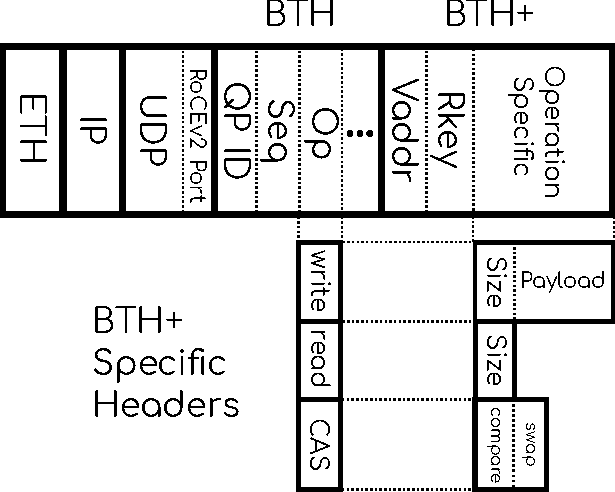
\includegraphics[width=0.485\textwidth]{fig/rocev2.pdf}
  \vskip -0.5em

    \caption{ RoCEv2 headers consist of an ethernet, ip, and
    udp header, a special udp port denotes that the packet
    is RDMA. The RoCE BTH header stores QP data, sequence
    numbers, flags, and operations. The BTH+ header follows
    and stores operation specific data such as virtual
    addresses, DMA size, and compare and swap payloads.
    }

    \label{fig:roce_header}
      \vskip -0.5em
\end{figure}

\sword uses the serialization provided by reliable
connections to prevent packet reordering after atomics have
been resolved.  As noted serialization on the switch is not
sufficient as reordering can occur on both the memory side
NIC, and PCIe bus(Figure ~\ref{fig:reorder}). Each reliable
connection is tracked by \sword which adds a new connection
to it's internal table when connections are set up, and
removes them on teardown, for a max of 4k connections. New
connections are detected by the first appearance of the QP
id. Each connection stores ip's, ports, ethernet addresses,
and rdma sequence numbers. Each packet on the connection is
tracked, and the switches internal sequence number for the
connection is incremented. Storing connection information
could lead to a potential memory bottle neck. Our aim is to
enable rack scale disaggregation where the total number of
cores (clients) is less thant O(1k). Here the few MB of
available switch memory is more than sufficient for storing
connection metadata.
%%
\begin{figure}[t]
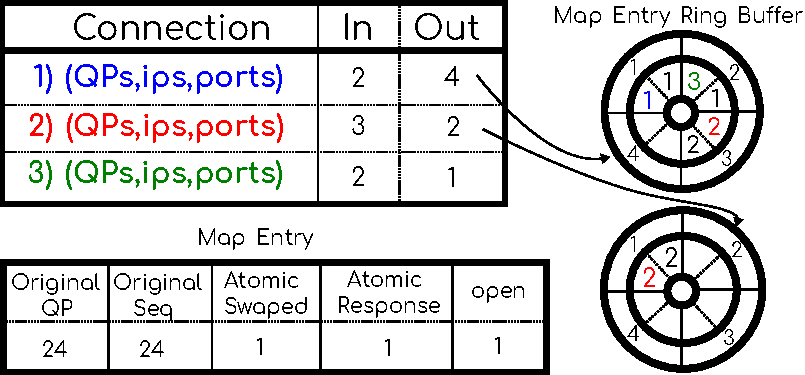
\includegraphics[width=0.485\textwidth]{fig/connection_multiplexing.pdf}
\vskip -0.5em

    \caption{ Queue pair mapping data structure. Each RC
    connection has metadata stored statically per
    connection. Sequence numbers are dynamic per connection,
    \sword stores both incomming and outgoing sequence
    numbers for each connection. Stubs for each outgoing
    request are stored in a fixed sized circular buffer.  }

    \label{fig:qp_mapping}
      \vskip -0.5em
\end{figure}

Each memory bound packet generates a map entry. The entry is
used to map packets back to their original connections. Each
map entry consists of the original sequence number, the
mapped sequence number, and the QP id of the original
connection. Hash entries are indexed into a ring buffer
array by their sequence number modulo the buffer size to
remove any hashing overhead. The buffer determines the max
number of in flight requests per qp (128 in \sword). One bit
marks if the map entry was transformed to a write from a
CAS. Our mapping data structure is shown in
Figure~\ref{fig:qp_mapping}.
%%
On mapping the invariant CRC (ICRC) of the RDMA packet must
be updated. Prior work has demonstrated that this is
possible in a programmable switch~\todo{cite}. We use RoCE
transport in which the ICRC is redundant after the ethernet
CRC. We turn off ICRC checks on both the sender and
receiver~\cite{switchml}.
%%
Tracking sequence numbers, and storing map entires is
sufficient for multiplexing RDMA packets.  To multiplex a
packet to another connection we update the packets ip
addresses, udp sender port, queue pair, and sequence number
then forward the packet as normal. Without applying these
updates the receiving side NIC will either reject the
packet, trigger go-back-n, or generate an error. 
%%
When a packet is mapped we increment the sequence number for
the receiving side QP.  Note that we do not need to
terminate connections at the switch but only maintain a
second set of sequence numbers for each connection as the
sender and receiver will become decoupled. When a response
packet is returned to {\sword} the sequence number is used
as an index back into the connections map entries, and the
mapping process is performed in reverse.

\subsection{Atomics to Writes}

Connection multiplexing enables serialized ordering for
requests from different clients. Two racing atomic
operations can be tie-broken in {\sword} have their response
values resolved and be modified from CAS to WRITE
operations. Changing atomics to writes significantly reduces
the operation bottleneck on a single address. 
%%
Transforming a CAS to a WRITE is reasonably straight forward
as the RoCE headers are similar. RoCE packets have two
headers BTH, and BTH+ headers, the BTH+ headers determine
the virtual addresses an operation executs on, the operation
itself, and its payload. Figure~\ref{fig:roce_packet}
details the difference between WRITE and CAS headers. When
mapping the virtual address and remote key remain the same.
We modify the opcode in the BTH header from WRITE to CAS
which instructs the memory side nic to treat the packet as a
write.  CAS is predefined to be 64 bit, so we install a
write header with a DMA length of 8, and a payload with the
tie breaker value. Note that the value set is application
specific. In the case of locking, the result is the locks
value after the operation is attempted. Finally the packet
length is truncated as write packets are 4 bytes shorter
than CAS packets.

\subsection{Ack de-coalescing}

Mapping RDMA connections back to their original clients is
not trivial. By default the RDMA protocol can coalesce ACKs
as an optimization. This is a performance advantage for a
single client as it reduces the overall number of packets,
but if an ack from a second client is coalesced with the
response the second client will not receive a response and
eventually time out. Leading to retransmissions and high
tail latencies. We detect coalescing on the switch by
monitoring response packets. If a higher number ack is
received we know by the guarantees of RC that the lower
packets operation was executed and it is safe to generate an
ACK for it. Using the mapped request for the lower packet we
generate an ACK and forward it to the other client. Multiple
acks can be coalesced so this processes is recursive when
ack coalescing is detected. This processes is not required
if response coalescing is turned off.

\subsection{Buffering}

\sword is designed for closed looped clients. Connection
remapping could require large amounts of buffering in
network if clients had many in flight requests spread across
multiple QP. Out of order requests would need to be buffered
prior to delivering them. Out of order packet delivery
triggers RoCE's go-back-n retransmission protocol.

\subsection{Steering}

Unlike connection multiplexing, steering does not modify the
RDMA operation. Steering is used when atomics are not
applied to a single address. The atomic bottleneck on
independent addresses is only half of that of reads and
writes, in most algorithms less than half of operations are
atomics, therefore the bottleneck is never reached. 
%%
We implement steering by maintaining a cache of centralized
data structure information, and data structure specific code
for resolving conflicts. When a packet arrives at the
switch, it is parsed and passed to the application specific
code. The cache is queried based on the virtual address, and
application data in the packet. If the packet requires an
update the virtual address in the BTH+ header is updated.
The cache is similarly updated based on the data structure
specific code.
%%
Reads and write are handled differently. Write contain
application specific data in the payload. This information,
along with the virtual address is usually sufficient to
identify the packet type specific to the application and
apply steering. While the semantics are application specific
in our evaluation we found it simple to do without making
modifications to the existing applications.
%%
Reads present a trickier problem. RDMA reads consist only of
a virtual address and a length. In some cases this may be
insufficient to identify if the packet needs to be steered,
or what the purpose of the packet is. In our evaluation we
keep an additional read cache which tracks the values and
purpose of recent writes (in our cases the old virtual
addresses of keys in a key value store.). If reads are
destined to a stale location, we steer them to the correct
location simply by modifying the virtual address.
%%
Our implementation of \sword requires no modification to the
existing systems, however we note that future systems
codesigend with \sword in mind could reduce the in network
memory footprint by fingerprinting their packets with id's
for {\sword}.

\subsection{Failure handling}

\sword\ collocates functionality---and therefore shares fate---with the
top-of-rack switch: if \sword\ fails, connectivity was already
disrupted (i.e., the ToR is down).  Hence, the fact that a
\sword\ failure will reset all remapped RDMA queue pairs to the
attached servers seems of little additional consequence.  In the case
of steering, however, we note that \sword\ does not maintain any hard
state: failure simply results in a performance hiccup if packet-level
connectivity can be maintained.  The upshot is that a complete
\sword\ failure does not introduce safety concerns in any event.

However, there are other failure scenarios to consider.  In
particular, we presume that the ToR sees the exact stream of packets
that will be received---and processed---by attached servers.
Unfortunately, this may not be true due to packet loss (e.g., due to
CRC failures or queue overflow) or even bugs on the server.  Of
course, these failure cases exist even without \sword, and Sherman and
Clover both provide their own error handling.  The key distinction,
however, is that \sword\ maintains a cache that may become
inconsistent with an attached server, which was previously the single
authority of both application and RDMA connection state.


At an application level, Clover never acquires any locks so failures
do not result in resource stranding, and Sherman periodically detects
if locks were kept by a dead client.  At the connection level they
both rely upon RDMA to provide reliable, in-order delivery of their
messages on a per-client basis and react to failed CAS operations by
retrying their operations.  {\sword} must therefore be able to detect
and properly handle packet retransmissions; in particular \sword\ must
not treat a retransmitted packet as a new operation.  Hence,
\sword\ tracks the most recent sequence number on each QP, the
transformation it applied (remapping or steering), and whether the
operation was ACK'd by the server.  Upon retransmission
\sword\ re-applies the previous transformation.

%QP ordering ensures retransmissions are , and RDMA
%go-back-$n$ is triggered if any message is lost.

\textbf{Enforcing ordering.}
Managing responses when mapping queue pairs is somewhat more complex.  If a
packet is dropped between \sword\ and a server and \sword\ maps a subsequent
request from a different client onto the same QP, the server will generate a
go-back-$n$ response and any other in-flight requests on that QP will become
invalidated.  Hence, when {\sword} sees a go-back-$n$ ACK, it triggers the same
mechanism used for ACK coalescing but in reverse: it broadcasts a go-back-$n$
ACK to all clients with outstanding messages.  While this approach amplifies the
performance impact of a lost packet, we expect such scenarios to be unlikely in
practice.  Indeed, no packet drops ever occurred between {\sword} and a server
during our experiments because our clients issue only closed-loop operations.

\textbf{Conflict avoidance.} Without queue-pair mapping, there are
fewer concerns at the connection level, but \sword\ must now be aware
of potential inconsistency between its cache and server state.
Concretely, in the case of Clover, it is possible for a linked list to
become ``broken''.  If \sword\ sees a client issue a \texttt{CAS(A,B)}
request (attempting to append node $B$ to the list at $A$) before
another issues \texttt{CAS(A,C)} (appending node $C$ to the
same---stale---tail), \sword\ will steer \texttt{CAS(A,C)} to
\texttt{CAS(B,C)}. If the \texttt{CAS(A,B)} operation is lost between
\sword\ and the server, \texttt{CAS(B,C)} will still succeed, causing
a broken chain: the pointer $A\rightarrow B$ does not exist but
$B\rightarrow C$ does, and {\sword} believes $C$ to be the tail.

In the normal case, the client will timeout and retransmit
\texttt{CAS(A,B)}, which \sword\ will identify as a retransmission and
\emph{not} steer to the ``new'' tail, thereby repairing the list.  (In
the mean time, the missing link is immaterial because
subsequent requests are being steered by \sword.)  If, however, the client
were to fail prior to retransmitting the CAS the chain will remain broken.
Here we use an out-of-band mechanism to repair the chain: on occasion
our control plane queries the switch to check for outstanding CAS
requests and simply retransmits them (spurious retransmissions are
handled gracefully by the server).  The trickiest case is if
\sword\ itself also fails in the mean time: we defer protecting
against this double-failure scenario to future work.





% {\sword} caches locks and forwards the result of locking
% operations to remote memory. Storing locks in switch memory
% enables 10's of millions of lock and unlock operations per
% second~\cite{netlock}. At these rates CAS on single
% addresses is the bottleneck. {\sword} serializes lock
% access and forwards the results to the servers, therefore
% the application CAS operation can be modified to a simple
% write as the result is known prior to arriving at the memory
% side NIC. On an individual QP this modification is safe --
% across QP however reordering can occur between the switch
% and memory. We therefore multiplex lock operations onto
% shared QPs.
% %%
% Swordbox manages reliable connections for all connected
% clients. When clients first connect {\sword} detect the
% connection startup and tracks the sequence numbers on that
% connection. The total number of active connections is
% tracked as well. When a lock acquire or release issued {\sword}
% take the lock address \textit{mod} it's address and assigns
% it to a connection. This ensures that all operations to the
% same lock are placed on the same reliable connection.
% %%
% When a CAS for a known lock passes through {\sword} it checks
% it's lock table and calculates the result of the locking
% operation, (aquired, released or failed). The RDMA packet
% then has it's operation value changed from CAS to Write, and
% is assigned to the downstream reliable connection the lock
% was mapped to. Each request must be multiplexed and
% demultiplexed, when a lock request is assigned to a stream
% it has it's QP, and sequence number updated so that the
% receving side NIC is unaware that any modification have been
% made in network. A stub of the mapping is stored with
% relation to the connection, when a response from the NIC
% returns from the switch the packet has it's sequence number
% mapped back to it's original value, and is mapped back to
% it's original sender. For each mapped request the switch
% must store both a sequence number and the id of the
% requesting client. 
% %%
% Our systems support only closed loop clients which issue one
% request at a time, and are guaranteed to retry requests lost
% in transit. Using this assumption the amount of state the
% switch needs to store is bounded by the number of clients.
% It must store a sequence number for each client QP, and
% stubs for each outstanding request. This requires at most 2
% 24 bit sequence number for each client.


% \subsection{Optimistic Concurrency}

% \subsection{Steering}

% Lock based data structures are limited under contention both
% by the rate at which locks can be acquired, and by the size
% of the critical section each client must execute. Under
% severe contention the critical section is the bottleneck.
% Optimistic strategies differ in that work completed in
% scratch memory, and then committed via an atomic operation
% like CAS. 

% Take for example a linked list which supports an append
% operation. Clients running append must first write the
% value of the node they wish to append, and then commit to
% the list by running a CAS which modifies the null pointer at
% the end of the list to then point to the new entry. Such
% strategies require no lock acquisition but still struggle
% under contetion. If the end of the list is continuously
% being appended to and multiple clients are in a race, one
% will succeed, the others will fail, need to traverse the
% list to the new tail, and reissue a request. 

% {\sword} is designed to entirely remove contention in
% optimistic concurrency schemes. As all requests are
% serialzed {\sword} can observer the most up to date location
% of the lists tail. We cache this value and use it to resolve
% conflicts. When requests arrive at sword which append to the
% tail of the list, the virtual address of the tail is stored
% for that key. This requires storing one 64 bit virtual
% address for each key in the key value store. While this
% overhead may seem large, {\sword} need only store hot keys.
% Uncontended keys can simply be written and read using
% clovers default protocol. When requests for a key arrive at
% {\sword} it looks up the value of the write and determines the
% location of the lists tail. If the request is pointing to
% the tail, the in network cache is updated and the request is
% forwared to memory with no modification. If the request is
% out of date (directed to an interior node of the list)
% {\sword} modifies the virtual address of the CAS and forwards
% it to the known tail location, updating it's own cache in
% the process.


\subsection{Example Systems}

We implement both of our contention reduction strategies in
two disaggregated systems Clover, and Sherman. 
%%
\textbf{Sherman}: is a B+ tree built for one sided RDMA.
Shermans core mechanism for mitigating write conflicts is a
lock table mapped to the memory side NIC. We emulate
Shermans lock table and demonstrate \sword's ability to
improve performance by placing the lock table in network and
mapping CAS operations to writes using our connection
remapping technique. We use our DPDK implementation of
\sword in our evaluation of Sherman.
%%
\textbf{Clover:}: is a key value store built for one sided
RDMA. One sided operations read and write updates to the
store by appending to keys structured as linked lists. Under
contention both reads and writes fail as the tail of the
lists move. We use \sword's ability to cache the most up to
date tail and steer requests to the correct location to
remove all contention from both reads and writes enabling
the performance of raw uncontended RDMA operations. Our
evaluation of Clover is performed using our P4
implementation of \sword.


% \textbf{sherman:} {{\sword}} assumes that locks are located at well known
% location. Logic for managing locks is application specific
% and implemented in {\sword}. No modification to the client is
% required as {\sword} operates directly on RDMA packets, using
% their QP id's and virtual addresses. In Sherman for instance
% locks are mapped to a special region of NIC memory with a
% well known virtual address range.

% \textbf{Clover:} This is the exact scheme Clover uses to
% handle writes to its persistent key value store. Clover
% operates well under read only workloads but struggles under
% contention as the tail of each list moves faster clients
% must repeatadly chase the tail pointer of the list, each
% read requiring a round trip.

% This strategy remotes all contention from Clover and
% requires not modifications to the application itself. A key
% aspect of this approach is that Clover has end to end
% recovery and does not rely on {\sword} to complete requests.
% If a key is not tracked by {\sword} then the request is
% forwarded directly to memory with no modifications. 

% Our
% prototype statically tracks hot keys, however a dynamic
% solution in which hot keys are detected via a count min
% sketch are well within the capabilities of future
% versions~\cite{switchml}.
